\documentclass[conference]{IEEEtran}

\usepackage{graphicx}
\usepackage{amsmath}
\usepackage{listings}
\usepackage{hyperref}
\usepackage{caption}
\usepackage{fancyhdr}
\usepackage{cite}
\usepackage{color}

\title{A Simple Convolutional Neural Network from Scratch}

\author{
\IEEEauthorblockN{Nguyen Nhat Anh - 2440057}
\IEEEauthorblockA{University of Science and Technology of Hanoi (USTH)\\
anhnn2440057@usth.edu.vn}
}

\begin{document}

\maketitle

\renewcommand{\thesubsection}{\alph{subsection}}

\makeatletter
\renewcommand{\@seccntformat}[1]{
  \ifcsname the#1\endcsname
    \csname the#1\endcsname.\hspace{0.5em}
  \else
    \csname name#1\endcsname:\hspace{0.5em}
  \fi}
\makeatother
\begin{abstract}
This report presents the implementation of a simple Convolutional Neural Network (CNNs) built entirely from scratch using only Python’s basic libraries, including \texttt{math}, \texttt{typing}, \texttt{PIL}, and \texttt{matplotlib}. No external numerical computing or machine learning frameworks were used, such as NumPy or TensorFlow. The model architecture includes up to two convolutional layers, a single max pooling layer, one dense output layer, and uses ReLU and softmax as activation functions. All hyperparameters are defined in an external configuration file. The model was evaluated on the MNIST handwritten digits dataset and achieved a classification accuracy of 78.75\%  on a small test subset. This implementation serves as a pedagogical tool to understand the core operations of CNNss without abstracted dependencies.
\end{abstract}

\begin{IEEEkeywords}
CNNs, MNIST, From Scratch
\end{IEEEkeywords}

\section{Introduction}

Image recognition plays an important role in many areas of science, especially in biology and microscopy. It is used for tasks like image filtering, segmentation, and object tracking. In microbiology, researchers rely on image analysis to automatically identify and count cells or bacteria from microscope images. This allows faster and more consistent analysis of large datasets, which would be time-consuming if done manually~\cite{shamir2010microscopy,uchida2018biology}.

To process and classify such image data effectively, Convolutional Neural Networks (CNNss) are commonly used. CNNss are inspired by the visual system of animals and are designed to learn visual patterns directly from raw pixel data. They are more efficient than fully connected networks because they use shared filters and local connections to detect features like edges or textures. Layers such as max pooling and activation functions like ReLU and softmax help the network learn better and make accurate predictions~\cite{matsugu2003face,aghdam2017CNNs}.

In this work, we use the MNIST dataset~\cite{lecun2010mnist}, a widely used collection of handwritten digit images. It contains 60{,}000 training and 10{,}000 test images, each in grayscale and sized 28$\times$28 pixels. MNIST is simple and well-structured, making it a good choice for testing basic neural networks. We build a simple CNNs from scratch using only standard Python libraries (\texttt{math}, \texttt{typing}, \texttt{PIL}, and \texttt{matplotlib})—without NumPy or deep learning frameworks. The network has fewer than three convolutional layers, one max pooling layer, and one fully connected layer. All configuration settings are loaded from a separate file. This project is intended to help learners understand the inner workings of CNNss by implementing every part manually.

\section{CNNs Approach}

Convolutional Neural Networks (CNNss) are a type of deep learning model particularly effective for image recognition tasks. Their architecture includes an input layer, a series of convolutional and pooling layers, and one or more fully connected layers for classification.

\subsection{Network Structure}
CNNss apply small filters (kernels) across the input image to extract spatial features, creating feature maps that highlight edges, corners, and textures. These feature maps are passed through nonlinear activation functions (e.g., ReLU) and pooled using techniques like max pooling to reduce dimensionality while preserving important patterns. The final feature representation is flattened and passed through dense layers to produce class scores via softmax activation \cite{shao2023mnist}.

\subsection{Key Characteristics}
CNNss differ from traditional fully connected networks due to:

\begin{itemize}
\item \text{Sparse interactions}: Each neuron is connected only to a small region of the input, reducing computation.
\item \text{Parameter sharing}: The same kernel weights are reused across all spatial locations, reducing the number of parameters.
\item \text{Pooling}: Pooling layers reduce the resolution of the feature maps while retaining essential information.
\item \text{Translation invariance}: The same feature can be recognized anywhere in the input image.
\end{itemize}

\subsection{Application to MNIST}
The MNIST dataset includes 28$\times$28 grayscale images of handwritten digits from 0 to 9. In our model, we use no more than two convolutional layers, one max pooling layer, and a fully connected output layer. Despite its simplicity, this structure is sufficient to capture key features such as stroke direction and shape. Hyperparameters like kernel size and number of filters are externally defined in a configuration file for flexibility.

\section{Materials and Methods}

\subsection*{a. Dataset}
The MNIST dataset (Modified National Institute of Standards and Technology) is a benchmark for evaluating handwritten digit recognition systems. It comprises 60,000 training samples and 10,000 test samples, each represented as a $28 \times 28$ grayscale image containing digits from 0 to 9 \cite{lecun2010mnist}.

The images have been centered and size-normalized within a $20 \times 20$ bounding box, and anti-aliased to preserve stroke information through grayscale values. This format allows for minimal preprocessing and is suitable for experimenting with pattern recognition and classification methods.

In our project, we used only a small subset of this dataset for demonstration purposes. The main goal was to validate the end-to-end data flow in a CNNs designed and implemented entirely from scratch.

\subsection*{b. Packages and Preprocessing}
To comply with the constraint of avoiding numerical libraries such as NumPy, we relied only on the following Python packages:
\begin{itemize}
    \item \texttt{math} – for logarithmic and exponential operations,
    \item \texttt{typing} – for annotating function arguments and improving code clarity,
    \item \texttt{PIL} – for reading and resizing PNG image files,
    \item \texttt{matplotlib} – for plotting and visualizing image data.
\end{itemize}

Each image was converted to a normalized 2D Python list (range: 0 to 1). Labels were extracted and matched manually. This minimal preprocessing pipeline reinforces the educational purpose of the implementation and avoids the use of automation tools like TensorFlow or Keras \cite{KerasUsers2017}.

\begin{figure} [!h]
    \centering
    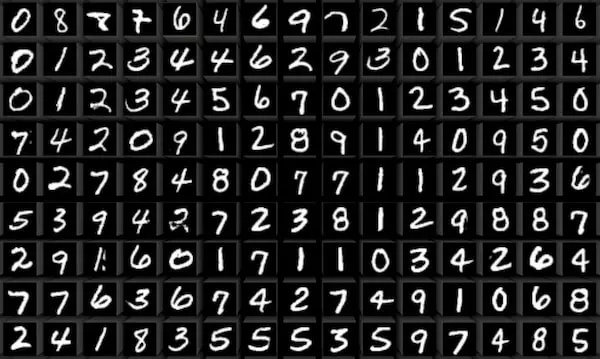
\includegraphics[width=0.8\linewidth]{image/example.png}
    \caption{Randomly selected samples.}
    \label{fig:enter-label}
\end{figure}

\subsection*{c. Mathematical Formulation and Model Architecture}
\textit{Mathematical Formulation}

The CNNs consists of two convolutional layers, one max pooling layer, a flattening stage, and a final dense layer with softmax activation.

\begin{itemize}
    \item \text{Convolution Layers}: Convolution computes feature maps using:
    \begin{equation}
        S(i, j) = \sum_{m=0}^{k-1} \sum_{n=0}^{k-1} I(i + m, j + n) \cdot K(m, n)
    \end{equation}
    Where $I$ is the input image patch, $K$ is the kernel, and $S(i, j)$ is the resulting activation. The ReLU activation function is applied element-wise:
    \begin{equation}
        \text{ReLU}(x) = \max(0, x)
    \end{equation}

    \item \text{Max Pooling}: To reduce the spatial dimension, we apply $2 \times 2$ max pooling:
    \begin{equation}
        P(i, j) = \max_{(m,n) \in R(i,j)} A(m, n)
    \end{equation}
    Where $A(m, n)$ represents activations from the previous layer and $R(i, j)$ is the pooling region.

    \item \text{Fully Connected Layer and Softmax}: After flattening the pooled feature maps, we compute the logits:
    \begin{equation}
        z_j = \sum_{i=1}^{n} x_i w_{ij} + b_j
    \end{equation}
    And apply the softmax function:
    \begin{equation}
        \hat{y}_j = \frac{e^{z_j}}{\sum_{k=1}^{10} e^{z_k}}
    \end{equation}

    \item \text{Loss Function}: The model uses cross-entropy loss:
    \begin{equation}
        L = -\sum_{j=1}^{10} y_j \log(\hat{y}_j)
    \end{equation}
    Where $y_j$ is the one-hot encoded ground truth label and $\hat{y}_j$ is the predicted probability \cite{goodfellow2016deep}.
\end{itemize}

Hyperparameters such as kernel size and number of filters were defined in a plain text configuration file, allowing for flexible changes without modifying the source code.

\textit{Model Architecture}

The designed CNNs consists of a minimal yet functional pipeline composed of one convolutional layer, one max pooling layer, and one fully connected (dense) layer.

\begin{itemize}
\item \text{Input Layer}: Each input image has a resolution of $28 \times 28$ pixels in grayscale, resulting in a single input channel ($\texttt{conv1\_channels} = 1$).

\item \text{Convolutional Layer}: A single convolutional layer is applied with a $3 \times 3$ kernel and a stride of 1. Given no padding, the output feature map size becomes $26 \times 26$:
\begin{equation}
(28 - 3 + 1) \times (28 - 3 + 1) = 26 \times 26
\end{equation}
Only one filter is used, resulting in a single output channel.

\item \text{Max Pooling}: A $2 \times 2$ max pooling layer is used, reducing the spatial resolution by half:
\begin{equation}
\left\lfloor \frac{26}{2} \right\rfloor \times \left\lfloor \frac{26}{2} \right\rfloor = 13 \times 13
\end{equation}
This significantly decreases the number of parameters and computation while preserving important features.

\item \text{Flattening}: The output of the pooling layer is flattened into a 1D vector of size:
\begin{equation}
13 \times 13 \times 1 = 169 \text{ neurons}
\end{equation}

\item \text{Dense Layer}: A fully connected dense layer with 10 units is applied to this 169-dimensional vector:
\begin{equation}
    y_j = \sum_{i=1}^{169} x_i w_{ij} + b_j
\end{equation}
\end{itemize}


\section{Results}

To evaluate the learning process and effectiveness of the implemented CNNs, we conducted training over 100 epochs using a subset of the small MNIST dataset. As the model was built without external frameworks and relied on forward-only propagation, weights were updated manually using a custom training loop.

The classification performance reached an accuracy of \textbf{78.75\%} on the test subset. Although the model architecture was minimal, this result confirms that the fundamental components—convolution, pooling, flattening, and classification—can be correctly implemented from scratch.

\begin{table}[h]
\centering
\caption{Training Loss at Key Epochs}
\label{tab:loss}
\begin{tabular}{|c|c|}
\hline
\textbf{Epoch} & \textbf{Loss} \\
\hline
10 & 24.3245 \\
20 & 11.3777 \\
30 & 6.1811 \\
40 & 4.0446 \\
50 & 3.0169 \\
60 & 2.4203 \\
70 & 2.0288 \\
80 & 1.7508 \\
90 & 1.5425 \\
100 & 1.3801 \\
\hline
\end{tabular}
\end{table}

Figure~\ref{fig:loss_curve} shows the training loss curve over 100 epochs. The loss decreased steadily, confirming that the model learned useful features during the training process.

\begin{figure}[!h]
\centering
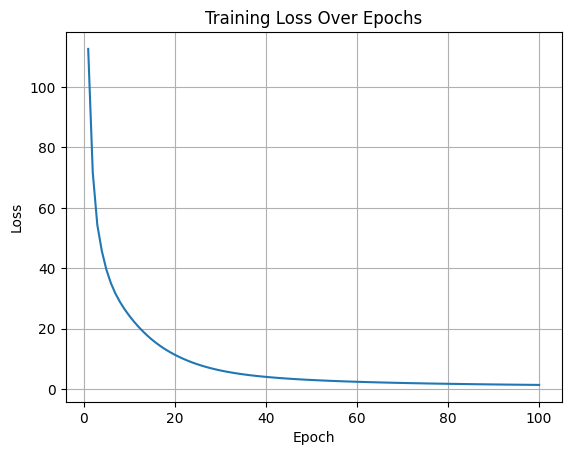
\includegraphics[width=0.75\linewidth]{image/loss.png}
\caption{Training loss over 100 epochs.}
\label{fig:loss_curve}
\end{figure}

These results demonstrate that even with manually implemented components and basic preprocessing, a small CNNs can still capture useful patterns and perform effective classification.

\begin{figure}[!h]
\centering
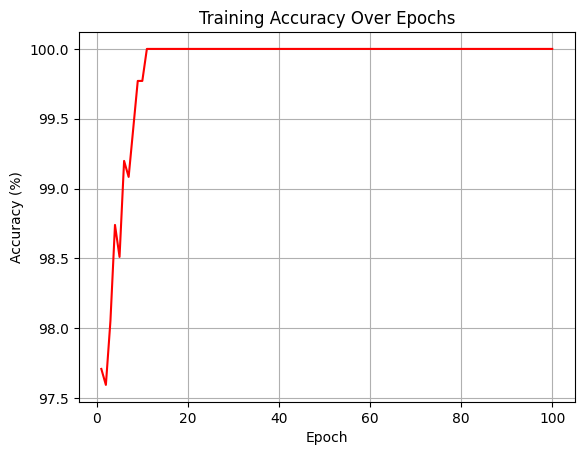
\includegraphics[width=0.75\linewidth]{image/accuracy.png}
\caption{The result of accuracy rate for the training set.}
\label{fig:loss}
\end{figure}

\begin{figure}[!h]
\centering

\label{fig:accuracy}
\end{figure}

\begin{figure}[!h]
\centering
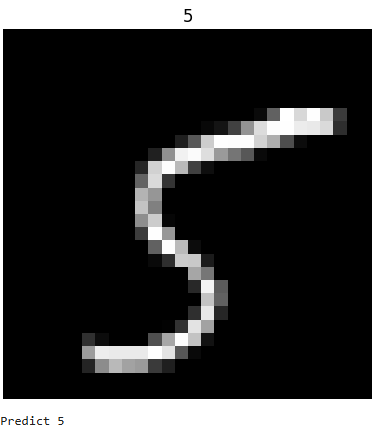
\includegraphics[width=0.45\linewidth]{image/5predict.png}
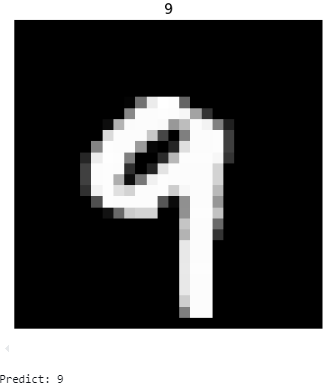
\includegraphics[width=0.45\linewidth]{image/9predict.png}
\caption{Example predictions: both digits are correctly classified by the CNNs as ``5'' and ``9'' respectively.}
\label{fig:predicted_examples_horizontal}
\end{figure}

Figure~\ref{fig:predicted_examples_horizontal} illustrates two sample predictions generated by the implemented CNNs. In both cases, the network correctly classified the input digits “5” and “9”. The model’s ability to predict accurately in such cases demonstrates its capacity to extract robust local features via convolution and retain discriminative patterns through pooling and fully connected layers. These results confirm that even a minimal architecture — with just one convolutional and one dense layer — can generalize reasonably well when trained on a representative subset of the MNIST dataset.

\section{Conclusion}

This project demonstrates the development of a simple Convolutional Neural Network (CNNs) entirely from scratch using only fundamental Python libraries, without the aid of NumPy or any high-level deep learning frameworks. The primary objective was to manually implement each critical stage of a CNNs pipeline — including convolution, activation, pooling, flattening, and dense output layers — in order to foster a deeper understanding of how such models operate at a low level.

The resulting network consists of a single convolutional layer, followed by a max pooling operation and a dense output layer with softmax activation. Evaluated on a small, balanced subset of the MNIST handwritten digits dataset, the model achieved an accuracy of 78.75\%. Although this performance is modest when compared to state-of-the-art models \cite{lecun2015deep}, it nevertheless confirms that basic network architectures can successfully extract and classify visual features with reasonable accuracy, even under tight computational and library constraints.

This outcome highlights both the educational value and practical limits of minimalist implementations. It showcases the potential of a basic CNNs to learn meaningful representations from visual data, despite the absence of parallel processing, optimized tensor libraries, or automatic differentiation. At the same time, the restricted model capacity and hand-coded backpropagation limit its ability to generalize, especially on more complex or noisy data.

Additionally, building the entire pipeline manually reveals the mechanics behind core operations such as convolution kernels, ReLU activation, max pooling, and softmax normalization. Each image is treated as a 2D grayscale matrix, and all mathematical computations are performed explicitly using loops and list manipulations. This approach promotes conceptual clarity and serves as an excellent pedagogical resource for those studying neural networks.

However, the experiment also underlines the drawbacks of using pure Python for deep learning — namely, slow training time and limited scalability. The project reinforces the necessity of optimized libraries and GPU support in real-world applications, especially when dealing with large-scale datasets or deeper architectures.

In future iterations, extending the model with additional convolutional layers, full gradient-based learning across all layers, and improved regularization (e.g., dropout) could significantly enhance accuracy and robustness. Furthermore, incorporating visualization techniques to inspect intermediate feature maps would provide valuable insight into how the network perceives different digit classes.


\section{Conclusion and Future Work}
We implemented a fully functional CNNs forward pipeline using core Python. Future improvements include implementing backpropagation, adding dropout regularization, and optimizing inference time. Additionally, visualizing feature maps across layers would enhance model interpretability.

\section*{Acknowledgment}
Special thanks to Assoc. Prof. Tran Giang Son for his continuous support, valuable guidance, and for proposing the minimalistic challenge that motivated us to deeply understand the core concepts.

\bibliographystyle{IEEEtran}
\begin{thebibliography}{00}

\bibitem{shamir2010microscopy}
L. Shamir, N. Orlov, D. Eckley, and I. G. Goldberg, ``IICBU-2008: A proposed benchmark suite for biological image analysis,'' \emph{Medical \& Biological Engineering \& Computing}, vol. 48, no. 9, pp. 939--949, 2010.

\bibitem{uchida2018biology}
S. Uchida, ``Image processing and recognition for biological images,'' \emph{Biology}, vol. 7, no. 3, p. 38, 2018.

\bibitem{matsugu2003face}
M. Matsugu, K. Mori, Y. Mitari, and Y. Kaneda, ``Subject independent facial expression recognition with robust face detection using a convolutional neural network,'' \emph{Pattern Recognition}, vol. 36, no. 2, pp. 303--314, 2003.

\bibitem{aghdam2017CNNs}
H. H. Aghdam and E. J. Heravi, \emph{Guide to Convolutional Neural Networks}. Springer, 2017.

\bibitem{lecun2010mnist}
Y. LeCun, C. Cortes, and C. J. Burges, ``The MNIST database of handwritten digits,'' [Online]. Available: \url{http://yann.lecun.com/exdb/mnist}, 2010.

\bibitem{KerasUsers2017}
F. Chollet et al., 
“Keras,” 
\url{https://keras.io}, 2017.

\bibitem{lecun2015deep}
Y. LeCun, Y. Bengio, and G. Hinton, ``Deep learning,'' \emph{Nature}, vol. 521, pp. 436--444, 2015.

\bibitem{goodfellow2016deep}
I. Goodfellow, Y. Bengio, and A. Courville, \textit{Deep Learning}. MIT Press, 2016.

\bibitem{shao2023mnist}
H. Shao, E. Ma, M. Zhu, X. Deng, and S. Zhai, ``MNIST Handwritten Digit Classification Based on Convolutional Neural Network with Hyperparameter Optimization,'' \emph{Intelligent Automation \& Soft Computing}, vol. 36, pp. 3595–3610, 2023. doi: \href{https://doi.org/10.32604/iasc.2023.036323}{10.32604/iasc.2023.036323}.

\end{thebibliography}
\end{document}
